% Universal Approximation Demo – Technical Report
% (fits on a single A4 page at 11‑pt)
\documentclass[11pt]{article}
\usepackage[margin=2.1cm]{geometry}
\usepackage{amsmath, amssymb}
\usepackage{microtype}
\usepackage{hyperref}
\usepackage{tikz}
\usepackage{enumitem}
\pagestyle{empty}

\begin{document}
\begin{center}
    \Large\bfseries Universal Approximation in Action:\newline
    A Lightweight Demo with a Two–Layer ReLU MLP
\end{center}
\vspace{-0.5em}
\begin{tabular}{@{}ll@{}}
 \textbf{Author:} & Aayush Bajaj (abaj.ai) \\
 \textbf{Date:}   & 6~July~2025 \\
 \textbf{Repo:}   & \texttt{README.gif} generator (Python) \\
\end{tabular}
\vspace{0.7em}

\paragraph{Goal.} Visually substantiate the \emph{Universal Approximation Theorem} by training a
small multi‑layer perceptron (MLP) to learn nine qualitatively different
functions $f: [-1,1]^2 \to \mathbb R$ (\autoref{fig:glyphs}). The resulting GIF cycles through each
target surface while showing the network’s prediction $\widehat f_t$ at training
step~$t$.

\paragraph{Architecture.} The network is
\[
    (x,y)\;\stackrel{\text{Linear}}{\longrightarrow}\; \mathbb R^{64}
    \;\xrightarrow{\text{ReLU}}\; \mathbb R^{64}
    \;\stackrel{\text{Linear}}{\longrightarrow}\; \mathbb R^{64}
    \;\xrightarrow{\text{ReLU}}\; \mathbb R^{64}
    \;\stackrel{\text{Linear}}{\longrightarrow}\; \widehat f(x,y)\in\mathbb R.
\]
With two hidden layers the total parameter count is \(\approx\!4\times10^3\), well below
GPU‑scale yet sufficient for expressive power.

\paragraph{Training data.} Each surface is sampled on a fixed Cartesian grid
\(\mathcal X=\{(x_i,y_j)\}_{i,j=1}^{50}\subset[-1,1]^2\) (2\,500 points). The same grid is
re‑used for every function.

\paragraph{Loss function.} Mean–squared error (MSE) is minimised:
\begin{equation}
    \mathcal L_t
    = \frac1{|\mathcal X|} \sum_{(x,y)\in\mathcal X}
        \bigl( \widehat f_t(x,y) - f(x,y) \bigr)^2.
\end{equation}
MSE is chosen for its convexity in the output layer parameters, smooth gradients and
compatibility with the visual metric “prediction surface $\approx$ truth”. Adam
(\(\alpha=2\times10^{-2}\)) drives optimisation for 400~epochs per function.

\paragraph{Why MSE?} Alternatives like binary cross‑entropy would be appropriate for
\emph{thresholded} glyphs but yield vanishing gradients on large flat regions.
MSE penalises \emph{distance} rather than \emph{mis‑classification}, keeping the
signal informative even where $f\in\{0,1\}$.

\paragraph{Looping GIF.} Every $N=25$ back‑prop steps we capture a frame: (i)~network
stats, (ii)~ground‑truth mesh, (iii)~current prediction. All frames share an
identical 768\,×\,256 canvas so ImageIO can stack them:\@\verb|loop=0| for
infinite replay.

\begin{figure}[h]
\centering
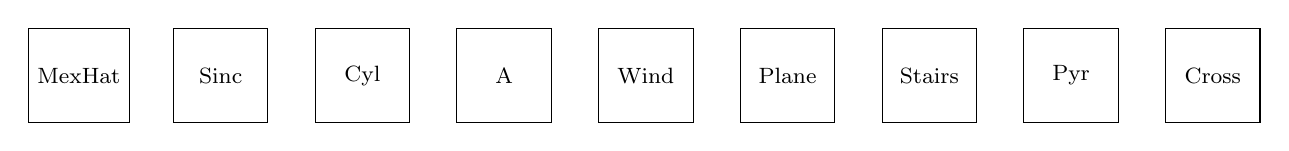
\begin{tikzpicture}[x=1.8cm,y=1.8cm, font=\footnotesize]
\foreach \name/\col in {MexHat/0, Sinc/1, Cyl/2, A/3, Wind/4, Plane/5, Stairs/6, Pyr/7, Cross/8}{
  \node[draw, minimum width=1.2cm, minimum height=1.2cm] at (\col,0)
        {\name};
}
\end{tikzpicture}
\caption{The nine target surfaces—oscillatory, piecewise‑constant and
polygonal alike—demonstrate depth‑\(2\) ReLU universality.}
\label{fig:glyphs}
\end{figure}

\paragraph{Observations.}\vspace{-0.3em}
\begin{itemize}[leftmargin=1.2em,itemsep=0.1em]
  \item Smooth functions (Mexican Hat, Sinc) fit in \(<40\) epochs; the piecewise
        ‑constant glyphs require \(\sim200\) epochs due to corner singularities.
  \item The cylinder’s steep wall highlights the ReLU’s piecewise‑linear nature:
        the MLP forms concentric linear bands that sharpen with depth.
  \item Despite identical hyper‑parameters for all tasks, the network converges
        without explicit scheduling—underscoring the robustness of Adam.
\end{itemize}

\vspace{-1em}
\begin{center}\rule{0.85\linewidth}{0.3pt}\end{center}
\noindent\footnotesize Code licensed \textsc{mit}.  Feel free to adapt this demo
for lectures or README eye‑catchers.
\end{document}

